%=========================================================================
% http://toms.acm.org/Authors.html
% ispell -p ./dictionary/dico.txt ortho_mads.tex
\documentclass[12pt,english]{article}

% \usepackage{pslatex}
% \usepackage{colortbl}
% \usepackage{graphicx}
\usepackage[english]{babel}
\usepackage[latin1]{inputenc}
\usepackage{amsmath}
\usepackage{amssymb}
\usepackage{epsfig}
\usepackage{colortbl}
\usepackage{moreverb}
\usepackage{pgf}
\usepackage{rotating}
\usepackage{array}
\usepackage{geometry}
\usepackage{times}
\def\no{\noindent}
\def\R{{\mathbb{R}}}
\def\Re{{\mathbb{R}}}
\def\N{{\mathbb{N}}}
\def\Z{{\mathbb{Z}}}
\def\Q{{\mathbb{Q}}}
\def\U{{\mathbb{U}}}
\def\demo{{\em Proof. }}
\def\mybox{\hfill{$\hbox{\vrule height4pt width4pt}$}}
\newcommand{\argmin}{\mathop{\mathrm{argmin}}}
\newcommand{\argmax}{\mathop{\mathrm{argmax}}}
\newcommand{\round}{\mathop{\mathrm{round}}}
\newcommand{\myst}{\mathop{\mathrm{s.t.}}}
\def\myif{\textbf{if }}
\def\myor{\textbf{or }}
\def\myelse{\textbf{else }}
\def\mygoto{\textbf{goto }}
\newtheorem{Def}{Definition}[section]
\newtheorem{Lem}[Def]{Lemma}
\newtheorem{Prop}[Def]{Proposition}
\newtheorem{Th}[Def]{Theorem}
\newtheorem{Cor}[Def]{Corollary}
\newtheorem{Res}[Def]{Result}
\newtheorem{Ex}[Def]{Example}
\newtheorem{Claim}[Def]{Claim}
\usepackage{xspace}
\definecolor{Red}{rgb}{.9,0.2,0.2}
\definecolor{lightred}{rgb}{1.0,0.9,0.9}
\definecolor{lightgreen}{rgb}{0.9,1.0,0.9}
\definecolor{lightblue}{rgb}{0.9,0.9,1.0}
\definecolor{lightcyan}{rgb}{0.8,1.0,1.0}
\definecolor{lightmagenta}{rgb}{1.0,0.5,1.0}
\definecolor{lightyellow}{rgb}{1.0,1.0,0.8}
\definecolor{yellow}{rgb}{1.0,1.0,0.0}
\definecolor{gris}{rgb}{0.4,0.4,0.4}
\newcommand{\Biz}[1]{\noindent \sethlcolor{gris}\hl{#1}}
\newcommand{\Charles}[1]{\noindent \sethlcolor{lightmagenta}\hl{#1}}
\newcommand{\John}[1]{\noindent \sethlcolor{lightcyan}\hl{#1}}
\newcommand{\Seb}[1]{\noindent \sethlcolor{yellow}\hl{#1}}
\def\boxwidth{12.4cm}
\geometry{letterpaper, tmargin=4cm, bmargin=3cm, lmargin=3.4cm, rmargin=3.4cm}
\setlength{\tabcolsep}{2.5pt}

%\newcommand{\nomad}{{\sc Nomad}\xspace}
\newcommand{\nomad}{NOMAD\xspace}
%\newcommand{\mads}{{\sc Mads}\xspace}
\newcommand{\mads}{MADS\xspace}
%\newcommand{\gps}{{\sc Gps}\xspace}
\newcommand{\gps}{GPS\xspace}
%\newcommand{\orthomads}{{\sc OrthoMads}\xspace}
\newcommand{\orthomads}{OrthoMADS\xspace}
%\newcommand{\ltmads}{{\sc LT-Mads}\xspace}
\newcommand{\ltmads}{LT-MADS\xspace}
%\newcommand{\bimads}{{\sc BiMads}\xspace}
\newcommand{\bimads}{BiMADS\xspace}
%\newcommand{\psdmads}{{\sc PsdMads}\xspace}
\newcommand{\psdmads}{PSD-MADS\xspace}
%\newcommand{\pmads}{{\sc pMads}\xspace}
\newcommand{\pmads}{p-MADS\xspace}
\newcommand{\coopmads}{COOP-MADS\xspace}

\newcommand{\bb}{blackbox\xspace}
\newcommand{\BB}{Blackbox\xspace}
\newcommand{\bbs}{blackboxes\xspace}
\newcommand{\search}{{search}\xspace}
\newcommand{\poll}{{poll}\xspace}
\newcommand{\Poll}{{Poll}\xspace}

\title{
    Algorithm xxx: NOMAD: Nonlinear Optimization with the MADS algorithm
    %\thanks{
    %  Work of the first author was supported by
     % {\sc Fcar} grant  {\sc Nc72792},
     % {\sc Nserc} grant 239436-05,
     % {\sc Afosr} FA9550-07-1-0302,
     % the Boeing Company, and ExxonMobil Upstream Research Company.
   % }
}
\author{
  S\'ebastien Le Digabel
  \thanks{{\sc gerad}
          and D\'epartement de math\'ematiques et de g\'enie industriel,
          Ecole Polytechnique de Montr\'eal,
          C.P. 6079, Succ. Centre-ville,
          Montr\'eal, Qu\'ebec H3C 3A7 Canada,
          www.gerad.ca/Sebastien.Le.Digabel,
          email: Sebastien.Le.Digabel@gerad.ca}
}

%=========================================================================
\begin{document}
\setcounter{page}{0}

%=========================================================================
\label{sec-front}
%=========================================================================

\thispagestyle{empty}
\maketitle
\thispagestyle{empty}

%=========================================================================
\section*{Using \nomad}
\label{sec-use}
%=========================================================================

This document is not the user manual of \nomad which
 is included in the \nomad package on the internet~\cite{Le09a}.
This section gives instructions to get quickly started with the optimization of
     a \bb problem.
Once installed, \nomad is easy to use as most of the parameters
  have defaults. In fact all algorithmic parameters have defaults
  and for a first try, only the parameters describing the problem
  are necessary.

 There are two modes for using \nomad.
 In batch mode, the \bb problem corresponds to a separated program
 that the \nomad executable will launch via system calls and temporary files.
 The other mode is the library mode: The user programs and links its problem
   directly with the \nomad static library
   (provided with the \nomad package).
 The library mode is a more advanced mode and the user has to learn the
   \nomad function prototypes and how to link its own code with the library.
This user code has typically to be written in C++,
  but examples in the \nomad package show
  programs using the library mode with a Windows DLL coded in Delphi,
  and a mini-application written in FORTRAN.
For problems which are not costly to compute,
 the execution is much faster because no temporary files are created.
For costly \bb problems, there is no speed gain by using the library mode.
Also, if the problem has hidden constraints,
   violating them may possibly interrupt the whole \nomad execution,
   unless these violations are detected and if
   exceptions are thrown by the user.
 In batch mode, when hidden constraints are violated, and if this crashes the \bb,
   then \nomad will simply ignore the corresponding evaluations.

 This section focuses on the batch mode and is based on the following
   academic problem taken from~\cite{HeFu06} with $n=5$:

\bigskip

\begin{equation}
  \min\limits_{
      \begin{subarray}{c}
        x \in  \R^5
      \end{subarray}
    } f(x)=- \left|   \frac{\sum\limits_{i=1}^{5}\cos^{4} x_{i} -
              2 \prod\limits_{i=1}^{5} \cos^{2}x_{i}}
              {\sqrt{\sum\limits_{i=1}^{5}ix_{i}^{2}}}   \right|$$

   $$\mbox{subject to} \left\{\begin{tabular}{rl}
     $-\prod\limits_{i=1}^{5}x_{i}+0.75 \leq 0$ \\
     $\sum\limits_{i=1}^{5}x_{i}-37.5\leq 0$ \\
     $0 \leq x_i \leq 10$,& $i=1,2,...,5$.
     \end{tabular}
   \right.
\label{ex-problem}
\end{equation}

  %----------------------------
  \subsection*{Installation}
  %----------------------------

  \nomad is available through three packages, for Windows, Mac, and Linux/Unix.
  After downloading the adequate file, the user must install it.
  On Windows, an installer program automatically
   copies the pre-compiled executables and libraries, which are then ready to use.
  On Mac, the files with executables and libraries are available inside
    a disk image.
   On Linux and Unix, the user has to compile the code with the \texttt{install}
   script.
  Note that the compilation of the source code is also possible on Mac and Windows,
    if a C++ compiler is installed.
  Any C++ compiler should work
    as \nomad has been developed with Linux
    without non-standard libraries and with the \texttt{-ansi} and \texttt{-pedantic}
    options of \texttt{gcc}, for the scalar version.
  For Windows systems, \nomad has been designed to compile with
    the \texttt{minGW} compiler and Microsoft Visual C++ 2008.
  For the parallel version, the standard level depends on which MPI implementation
    is used.

  Once the installation step has succeeded, the user is invited to define its
    own environment
    variables to ease the access to the software
    and the compilation of the examples.

  %--------------------------------------
  \subsection*{Defining the problem}
  \label{sec-bb}
  %--------------------------------------

In batch mode, the problem reduces to the \bb executable
  and possibly to bounds on the variables.
Bound constraints are the only constraints that may be indicated outside
  the \bb.
Of course the \bb is still valid if it codes directly its own bounds,
  but \nomad will be more efficient with that knowledge.
There are two ways to specify the bounds: They may be directly specified
  in the parameters file or entered in two text files that \nomad will load.

The \bb executable has very few design constraints to respect:
  It may be coded in any language as long as it is callable from a
  command line.
For example, a \bb that executes itself from a graphical user interface is
  not valid for \nomad.
For such applications, the user must code a wrapper program that will
  be callable from the
  command line.

More than one executable can be used.
 This is relevant when the first executable displays EB constraints, and
 if one of
 these constraints is violated: In that case,
  \nomad will not call the other executables.
We assume from now on that only one executable is used.
 \nomad executes the \bb with system calls. It indicates a trial point
   $x$ at which the \bb must compute the functions $f$ and $c_j$'s.
 The point $x$ is given in a text file containing the coordinates
   separated by spaces.
 Figure~\ref{fig-bb} shows an example on how a \bb should be called.
 The name of this file is given as an argument in the command call.
 The results of the functions computations have
 to be displayed on the standard output by the \bb, and
 it is preferable to display these outputs with a good numerical precision.
 The choice for the display order
   is left to the user and will be specified in the parameters file.

 If the \bb needs to create temporary files, those should be created with
     unique names to be compatible with the parallel versions of \nomad.
     To do so, it is possible to make \nomad include a unique tag
           in the input file.
Note also that %, as explained in Section~\ref{sec-scaling},
          if the problem has scaling issues,
          the user can scale the problem variables
          directly into the \bb or with the \texttt{SCALING} parameter.

%---------------------------------------------%
%  BB FIGURE
%---------------------------------------------%
\begin{figure}
\begin{center}
  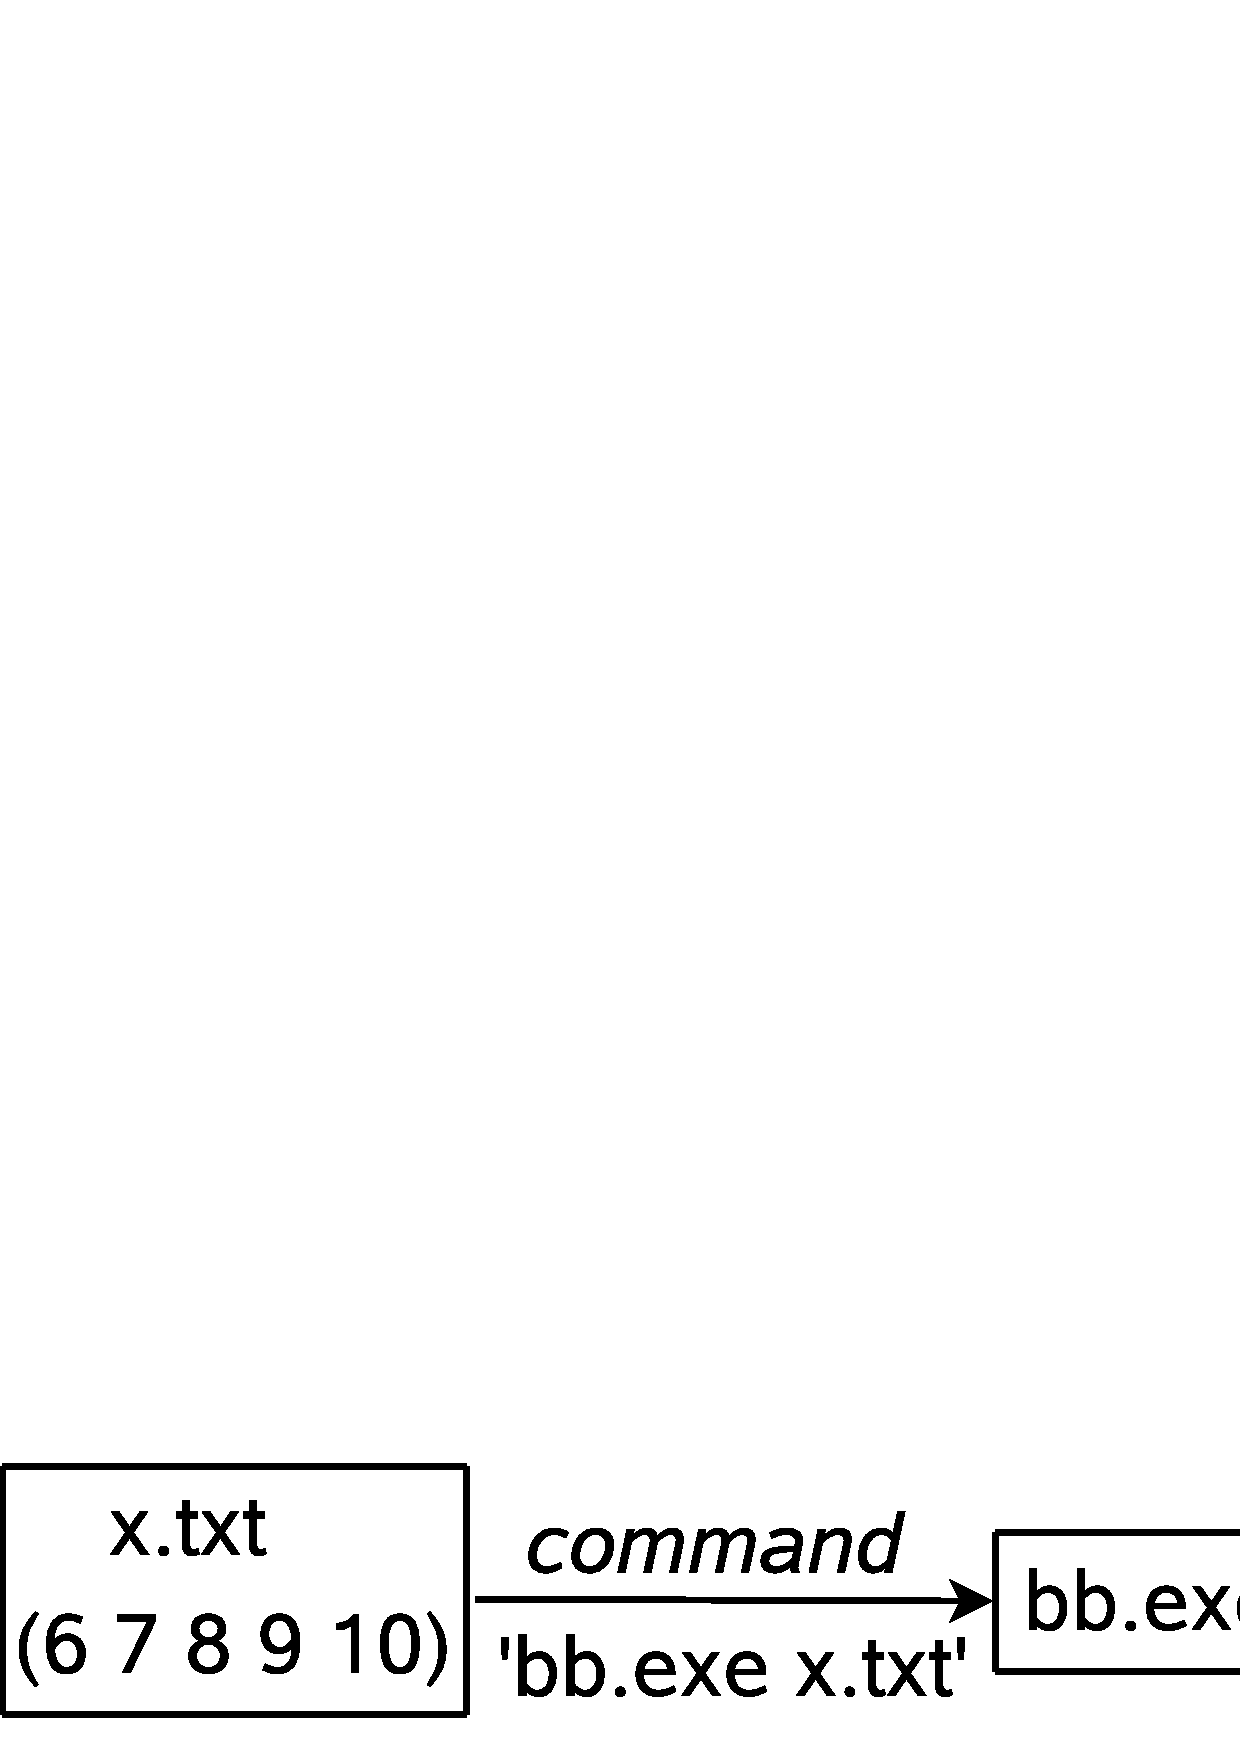
\includegraphics[width=14cm]{bb}
\end{center}
\caption{Example of a \bb call sequence. The \bb program is \texttt{bb.exe},
              which is executed with the command line instruction
              \texttt{`bb.exe x.txt'} where \texttt{x.txt} is a text file containing
              a trial point coordinates. The \bb has first to read this file and then
              to compute the functions defining the problem. When this is done,
              the function values are displayed on the standard output.
              The values given here are consistent with
              Problem~(\ref{ex-problem}).
              }
\label{fig-bb}
\end{figure}
%---------------------------------------------%

%---------------------------------------------
\subsection*{Creating a parameters file}
%---------------------------------------------

\nomad possesses several parameters for a great flexibility.
   However, all the algorithmic parameters have default values allowing
   out-of-the-box use without deep knowledge of the software and of the
   algorithm.

 Only the most important parameters are evoked in this paper.
 All the parameters are detailed in the user guide, and
  it it also possible
  to display help on them directly from the \nomad executable, by indicating
  a keyword after a \texttt{-h} flag.
  For example, entering the command \texttt{`nomad -h mesh'}
    will display all the parameters related to the mesh.
  Some other keywords such as \texttt{constraints} or \texttt{stop}
  are also defined to give special help.

It is indicated here how to create the basic parameters file necessary to launch \nomad
 on Problem~(\ref{ex-problem})
 which \bb executable has been coded according to Section~\ref{sec-bb}.
This basic file only needs to specify the problem characteristics.

\nomad automatically defines the problem directory as the one where the parameters file
  is located.
All the file names correspond to files
  (inputs or outputs) that must be located
        relatively to the problem directory, though it is possible to define
        these locations with absolute paths.
It is then adequate to create the parameters file at the same location than the \bb program.

The file associated to Problem~(\ref{ex-problem}) is shown in Figure~\ref{fig-ex-param}.
The starting point in the figure is defined to be $x_0=(6~7~8~9~10)^T$.
    It could also have been specified with a text file containing the coordinates
    separated with spaces or line breaks.
Notice the use of parameter \texttt{BB\_OUTPUT\_TYPE} to define
  what are the output types of the \bb. Here it indicates that the
  last value displayed at the execution of \texttt{bb.exe} is the objective value
  to minimize and the two first values correspond to the constraints
  $c_1(x) \leq 0$ and $c_2(x) \leq 0$.
The keyword \texttt{CSTR} has been used, meaning that \nomad will treat these constraints
  with the default PB constraints handling strategy. % (see~\ref{sec-cstr}).

  Bounds may be indicated directly into
         the parameters file or with additional text files.
        For Problem~(\ref{ex-problem}), one line in the example
        of Figure~\ref{fig-ex-param} is sufficient to specify them.

In the example, no algorithmic parameters are defined.
In particular no
       stopping criterion is indicated, which will let \nomad run until
       the mesh size parameter $\Delta_k^m$ drops below the \nomad default precision
       of $10^{-13}$.

%---------------------------------------------%
%  PARAMETERS EXAMPLE
%---------------------------------------------%
\begin{figure}[ht]
\begin{center}
\begin{boxedverbatim}
DIMENSION      5
BB_EXE         bb.exe
BB_OUTPUT_TYPE CSTR CSTR OBJ
x0             ( 6 7 8 9 10 )
LOWER_BOUND    * 0.0
UPPER_BOUND    * 10.0
\end{boxedverbatim}
\end{center}
\caption{A basic parameters file for Problem~(\ref{ex-problem}),
              assuming that the \bb executable created accordingly to
              Section~\ref{sec-bb} is named \texttt{bb.exe} and is located
              in the same directory than the parameters file.}
\label{fig-ex-param}
\end{figure}
%---------------------------------------------%

%------------------------------------------------
\subsection*{Running \nomad}
%------------------------------------------------

In batch mode, \nomad is executed with the command
  \texttt{`nomad param.txt'} where \texttt{param.txt} is the parameters file.
A stopping criteria on the maximum number of \bb evaluations is added
  to the parameters file of Figure~\ref{fig-ex-param} to show
  an example of the \nomad output on Problem~(\ref{ex-problem})
  with a reasonable length.
This criteria corresponds to the
   \texttt{MAX\_BB\_EVAL} parameter and it is set to 300
   evaluations with the instruction
   \texttt{`MAX\_BB\_EVAL 300'} in the parameters file.
Several stopping conditions are available in addition to the maximum number
           of \bb evaluations tested here.
 For example, minimum mesh or poll sizes can be specified
          as well as a maximum time limit. \nomad can also be interrupted when
          the objective value reaches a given limit or simply
          after a feasible solution has been found.
 Type the command \texttt{`nomad -h stop'} to
           see a complete description on all the parameters related
           to the stopping conditions.

%---------------------------------------------%
%  NOMAD RUN EXAMPLE
%---------------------------------------------%
\begin{figure}[ht]
\begin{scriptsize}
\begin{center}
\begin{boxedverbatim}
NOMAD - version 3.4.1 - www.gerad.ca/nomad

Copyright (C) 2001-2010 {
        Mark A. Abramson     - The Boeing Company
        Charles Audet        - Ecole Polytechnique de Montreal
        Gilles Couture       - Ecole Polytechnique de Montreal
        John E. Dennis, Jr.  - Rice University
        Sebastien Le Digabel - Ecole Polytechnique de Montreal
}

Funded in part by AFOSR and Exxon Mobil.

License   : `$NOMAD_HOME/src/lgpl.txt'
User guide: `$NOMAD_HOME/doc/user_guide.pdf'
Examples  : `$NOMAD_HOME/examples'
Tools     : `$NOMAD_HOME/tools'

Please report bugs to nomad@gerad.ca

MADS run {

        BBE     OBJ

        6       -0.09090074078
        13      -0.093399105
        115     -0.1080484746
        160     -0.1187621478
        161     -0.1525259466
        174     -0.1647326914
        175     -0.194081576
        187     -0.1963317314
        218     -0.2081777291
        228     -0.2191602101
        230     -0.2195574212
        231     -0.2464497881
        283     -0.25334522
        296     -0.2601065155
        300     -0.2601065155

} end of run (max number of blackbox evaluations)

blackbox evaluations   : 300
best infeasible solution: ( 0.125 0 0 0 0 ) h=0.75 f=-24.00193288
best feasible solution  : ( 3.25 3 5.75 3 1.5 ) h=0 f=-0.2601065155
\end{boxedverbatim}
\end{center}
\end{scriptsize}
\caption{\nomad output on Problem~(\ref{ex-problem})
             with parameters of Figure~\ref{fig-ex-param}.
%Values have been rounded to 4 decimals to fit in the page width.
        }
\label{fig-ex-run}
\end{figure}
%---------------------------------------------%

The output of \nomad for Problem~(\ref{ex-problem}), with
 parameters from Figure~\ref{fig-ex-param}, is displayed in Figure~\ref{fig-ex-run}.
The amount of displayed information is dictated
          by the \texttt{DISPLAY\_DEGREE} parameter
          with values ranging from
          0 (no display at all) to 2 (full display).
During the algorithm execution, with the default display degree,
       information is given every time a new feasible iterate is found.
       In the example of Figure~\ref{fig-ex-run}, the displayed information
       is the number of \bb evaluations and the objective value.
 This information is completely customizable with the
         \texttt{DISPLAY\_STATS} parameter which recognizes special keywords
         such as \texttt{OBJ} for the objective value,
         \texttt{SOL} for point coordinates,
         or \texttt{TIME} for the elapsed time.
 Understanding the use of this parameter
         allows for example to directly output \LaTeX~entries.
  Notice the final solutions displayed by the execution and the fact that
    the best feasible point has a constraint violation
    $h$ of 0 while the best infeasible point
    as a strictly positive value for $h$.
  In addition, the first success appears after 6 evaluations: The starting point
    was not feasible and it took \nomad 6 evaluations to get
    its first feasible solution with a value of $\simeq -0.09$
    for the objective.

  It is possible to generate up to three output files: A history file,
      containing all the \nomad trial points, a solution file with the final
      $\hat{x}$ solution (if feasible), and a configurable file
      containing all the successes with the same logic as the
      \texttt{DISPLAY\_} \texttt{STATS} parameter.

  Finally the \texttt{CACHE\_FILE} parameter
    may be specified to create and maintain a binary file
    containing all the evaluations.
  This file can then be used for other \nomad runs.

  %---------------------------------------
  \subsection*{Advanced use and flexibility in \nomad}
  \label{sec-advanced-use}
  %---------------------------------------

As already mentioned, there are a lot of parameters in \nomad.
The reader is invited to consult the detailed list of parameters in the
  user guide~\cite{Le09a} or to explore the output of the \texttt{`nomad -h'}
  command.

\nomad can minimize biobjective problems: It will then construct a list
  of undominated solutions which are an approximation of the Pareto front.
In order to define a biobjective problem, the user must simply
  define two \bb outputs with the keyword \texttt{OBJ}.
\nomad then automatically uses \bimads and
  launches a series of \mads runs.
There again, all the algorithmic parameters have default values and the
  advanced user can change them
  (enter \texttt{`nomad -h multi'} to display all these parameters).
 The most useful biobjective parameter is \texttt{MULTI\_OVERALL\_BB\_EVAL}
 which is the equivalent of \texttt{MAX\_BB\_EVAL} for single-objective optimization.
The \texttt{MAX\_} \texttt{BB\_EVAL}
  parameter  is still used in biobjective mode but corresponds
  to the maximum number of \bb evaluations for a single \mads run.

In order to improve performance, the user may try several strategies.
It would be too long to enumerate all these strategies in the present paper
  but here are
 some easy measures that can help.
If \nomad is used in batch mode
   on a network, the user should indicate a local directory
   (\texttt{/tmp} on Unix for example)
   where all the temporary files are created
(parameter \texttt{TMP\_DIR}).
This way, file manipulations will be faster.
This will however only improve performance for
  non-costly \bbs, when the cost of reading and writing
  files is non-negligible compared to the cost of the evaluations.

Other parameters may have a great impact on the quality of the solution: For example
  the starting point
  (\texttt{X0})
  or the value of the initial mesh size parameter
  (\texttt{INITIAL\_MESH\_} \texttt{SIZE}).
The parameter \texttt{SNAP\_TO\_BOUNDS} may also change performance.
It decides if trial points generated outside bounds are
  modified so that too large or too small coordinates are set
  to their bounds.
This strategy is used by default but it may be necessary for some problems
  to disable it.
The user may change the random seed used for the \ltmads directions (\texttt{SEED})
  or the Halton seed of the \orthomads directions (\texttt{HALTON\_SEED}).
The LH and VNS \search steps are also available via
 the parameters
 \texttt{LH\_SEARCH} and \texttt{VNS\_SEARCH}.
 The user must though be aware of the possible additional cost in terms of evaluations.
In some cases, scaling can also be a performance issue.

 Additional parameters may be used to indicate a surrogate function for the \bb.
Surrogate executables must have the same outputs as the true functions they substitute
and must be callable the same way.
Wishfully, they are also cheap to execute.

The library mode of \nomad offers even more flexibility and performance:
     Several functionalities can be redefined via the virtual functions of \nomad, but
     this mode is only accessible with a minimal knowledge of C++
     and object oriented programming.

In library mode the user must create a main function and link
  it with the \nomad static library file \texttt{nomad.a} (on Linux).
The \bb functions may be defined inside the code or as separated programs as
  in the batch mode.
A \texttt{NOMAD::Parameters} object must
  be constructed with the \texttt{set} methods
  included in the class interface.
Once the problem and the parameters are defined, a \texttt{NOMAD::Mads}
  object must be created
  and executed with \texttt{NOMAD::Mads::run()} or
  \texttt{NOMAD::Mads::multi\_run()} in the
  biobjective case.
Optimization results are accessible from \texttt{NOMAD::Mads} and
  \texttt{NOMAD::Stats} classes.

Here is a short list of functionalities available with
     the library mode: %As already mentioned in~\ref{sec-eval},
     users can preprocess the trial points before they are evaluated
     and give the evaluation points a priority for being evaluated.
Virtual customizable functions are also automatically
  called after each iteration and after each success
  (functions \texttt{update\_iteration()}
    and \texttt{update\_success()} from \texttt{NOMAD::Evaluator}).
Users can also code their own \search strategy. %as described in~\ref{sec-func}:
  To do so, they must design a subclass of the \texttt{NOMAD::Search} class and
    link an object of this class to the \texttt{NOMAD::Mads} object used to
    run the algorithm.
Virtual functions are also necessary to treat problems
  with categorical variables as they allow the user to define
  the neighborhoods of these variables.

For all these virtual functions, the user must be aware that
  modifying or generating new trial points may destroy
  the global convergence properties of the algorithm,
  as in the example 2.2 of~\cite{AuLe09}
  where a user-defined search leads to a point
  without any optimality property.
The main condition to ensure in any modification is
  that points remain on the mesh.
The function \texttt{NOMAD::Point::project\_to\_mesh()}
  is available for that purpose.
The decision to project points to the mesh is explicitely left
  to the user for a greater flexibility.

 Several examples are given in the \nomad package, illustrating various
            advanced situations in batch or library modes.
  For example, a multi-start based on LH sampling is given as well as a
    user \search strategy.
  Other examples show that \nomad can be interfaced with \bb problems
    that are coded in other languages: Such examples include
    AMPL~\cite{FoGaKe03a},
    MATLAB, GAMS~\cite{BrKeMe88a}, CUTEr~\cite{GoOrTo03},
    and an example where the \bb is a Windows dynamic library (DLL).
  Another example shows how to use \nomad version 3 with the previous version 2.


%=========================================================================
\bibliographystyle{plain}
%\bibliography{bibliography}

\begin{thebibliography}{1}

\bibitem{AuLe09}
C.~Audet and S.~Le Digabel.
\newblock The mesh adaptive direct search algorithm for periodic variables.
\newblock Technical Report G-2009-23, Les cahiers du GERAD, 2009.

\bibitem{BrKeMe88a}
A.~Brooke, D.~Kendrick, and A.~Meeraus.
\newblock {\em {GAMS}: A Users' Guide}.
\newblock The Scientific Press, Danvers, Massachusetts, 1988.

\bibitem{Le09a}
S.~Le Digabel.
\newblock {NOMAD} user guide.
\newblock Technical Report G-2009-37, Les cahiers du GERAD, 2009.

\bibitem{FoGaKe03a}
R.~Fourer, D.~M. Gay, and B.~W. Kernighan.
\newblock {\em {AMPL}: {A} Modeling Language for Mathematical Programming}.
\newblock Thomson/Brooks/Cole, Pacific Grove, California, second edition, 2003.

\bibitem{GoOrTo03}
{N. I. M.} Gould, D.~Orban, and {Ph.}~L. Toint.
\newblock {CUTEr} (and {SifDec}): a constrained and unconstrained testing
  environment, revisited.
\newblock {\em ACM Transactions on Mathematical Software}, 29(4):373--394,
  2003.

\bibitem{HeFu06}
A.~Hedar and M.~Fukushima.
\newblock Derivative-free filter simulated annealing method for constrained
  continuous global optimization.
\newblock {\em Journal of Global Optimization}, 35(4):521--549, 2006.

\end{thebibliography}
%=========================================================================
\end{document}
%=========================================================================
